This section presents our GPU porting approach, followed by our 
fine-grained data-management strategy designed to minimize host--device 
data movement.

\subsection{Porting Approach}
\label{sec:method-approach}

We ported LESGO using OpenACC directives with the NVHPC compiler and
bound batched cuFFT spectral transforms to the same CUDA streams as the
OpenACC kernels. We chose compiler directives over a low-level CUDA
rewrite because LESGO is an extensive, physics-validated codebase
actively maintained by user community extending the Fortran source.
Directive-based offloading preserves a single source tree in which the
CPU build remains reproducible and acts as our correctness reference.
This approach also aligns with established porting practices in
scientific computing, as demonstrated across atmospheric fluid
models~\cite{esclapez2025dales,lapillonne2014,govett2017nim} and other
production Fortran codebases~\cite{otero2019nek,caplan2019mas}.

The computational pattern across the code is uniform. The solver state
consists of dozens of persistent 3D Fortran arrays of $O(N^3)$ size,
including velocity components, velocity gradients, subgrid-scale (SGS)
stresses, and dealiased spectral scratch fields. Nearly every kernel
sweeps these fields with a triple-nested loop. While this uniformity
simplifies compute offloading, it heightens the penalty for poor data
placement because any unnecessary host--device synchronization transfers
$O(N^3)$ bytes.

\subsection{Data-Movement Bottlenecks}
\label{sec:method-problem}

We now quantify the limitations of the two dominant data-placement
strategies in directive-based ports.

\begin{figure}[h]
  \centering
  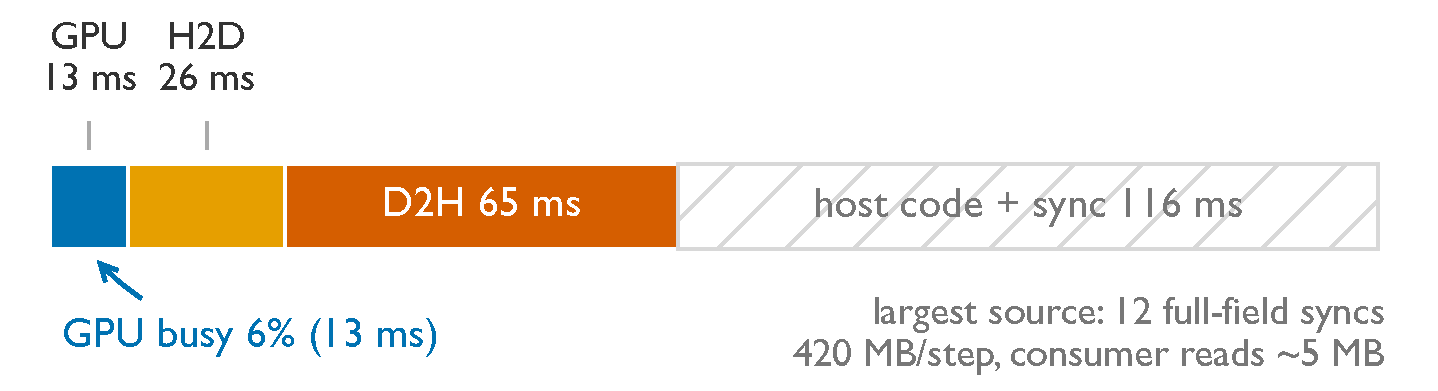
\includegraphics[width=\linewidth]{figs/fig_mirroring.pdf}
  \caption{Time-step breakdown under array mirroring on the reference case ($256^3$ cells, 4 A100 GPUs). Host--device transfers and host-side synchronization leave the GPU 94\% idle.}
  \label{fig:mirroring}
\end{figure}

% \vspace{0.08in}
\textbf{Array Mirroring.} When the solver state fits comfortably in device memory, mirroring every
host array on the device is an effective strategy, as all kernels can
move to the GPU and data returns to the host only for diagnostics and
checkpoints~\cite{esclapez2025dales,giorgetta2022}. LESGO, however,
does not fit this mold for two reasons. First, its state comprises
dozens of $O(N^3)$ fields plus $3/2$-padded spectral scratch, so
duplicating arrays that no kernel reads wastes device memory and increases the number of GPUs a
given grid requires. Second, several routines run slower on the GPU than
on CPUs, and should therefore remain on the host. Mirroring
consequently still requires PCIe transfers wherever these host-resident
routines consume solver state. On our reference configuration ($256^3$
grid with two wind turbines on 4 A100 GPUs), \texttt{Nsight Systems}
profiling reveals that only 13\,ms of a 220\,ms time step is spent on
GPU execution. PCIe transfers and host-side synchronization account for
the remaining 207\,ms, leaving the GPU \textbf{94\% idle}
(Fig.~\ref{fig:mirroring}). The dominant bottleneck is a full-field
synchronization of twelve $O(N^3)$ arrays (420\,MB per step).

% \begin{figure}[h]
% \centering
% 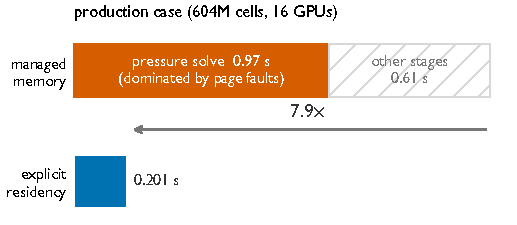
\includegraphics[width=\linewidth]{figs/fig_managed.pdf}
% \caption{Per-step time under CUDA managed memory versus explicit residency on the production case (604M cells, 16 A100 GPUs).}
% \label{fig:managed}
% \end{figure}

\vspace{0.08in}
\textbf{CUDA Managed Memory.} Managed memory minimizes initial porting
effort and underpins Fortran standard-parallelism
offloading~\cite{caplan2023dc}, making it an attractive default for
directive-based ports. However, evaluating CUDA managed memory
(\texttt{-gpu=mem:managed}) on the production benchmark
(Section~\ref{sec:setup}) across 16 A100 GPUs yields limited acceleration. 
Using \texttt{nsys} profiling, we found that
extensive page faults and data migration overheads inherent to
demand-paged unified memory~\cite{chien2019um} severely stall execution.

Both profiles point to the same root cause. After the compute kernels
move to the GPU, certain routines still execute on the host and demand
full-field data transfers to do so. Achieving high GPU efficiency therefore 
requires fine-grained, structure-aware control over data residency and
host--device transfer footprints.

\subsection{Consumer-Driven Explicit Residency}
\label{sec:method-taxonomy}

\begin{table*}[t]
\centering
\caption{Taxonomy of host--device coupling points in a pseudo-spectral
multiphysics LES solver and the data-residency strategies that resolve each class. 
% Naive costs are measured per step on the reference configuration [R] or the production case
% [P].
}
\label{tab:taxonomy}
\footnotesize
\renewcommand{\arraystretch}{1.2}
\rowcolors{2}{gray!12}{white}
\begin{tabular}{@{}
  >{\raggedright\arraybackslash}p{0.8in}
  >{\raggedright\arraybackslash}p{2.35in}
  >{\raggedright\arraybackslash}p{1.05in}
  >{\raggedright\arraybackslash}p{2.25in}@{}}
\toprule
Class & Instance in LESGO & Naive cost per step & Treatment \\
\midrule
Boundary plane & wall-stress model reads $u,v,w$ at the walls &
full fields, 420\,MB & \emph{slice} to wall planes, later
\emph{relocate} \\
Conditional & velocity gradients read by the CPU SGS fallback only &
9 fields, 315\,MB & \emph{gate} on the SGS model choice \\
Spectral mode & pressure zero-wavenumber recurrence (serial in $z$) &
3 full-field round trips & \emph{slice} to the DC column
($\sim$1\,KB) \\
Stale entry & \texttt{copyin} of pressure at solver entry &
34\,MB & \emph{slice} to a seeded ghost plane via \texttt{create} \\
Pipeline state & time integration and projection read $u,v,w$, RHS &
210\,MB & \emph{relocate}, keep the update pipeline
device-resident \\
Actuator & blade sampling and force projection & 2 full-field
crossings & \emph{relocate}, exchange $O(\text{blade points})$
(\S\ref{sec:opt-batch}) \\
Diagnostics & energy, divergence, checkpoint writes & 963\,MB 
& \emph{relocate} reductions, \emph{gate} output
steps \\
Serial chain & tridiagonal Thomas chains spanning ranks &
host-staged relays & \emph{relocate}, pipelined GPU-aware exchange
(\S\ref{sec:opt-tridag}) \\
Host physics & tabulated airfoil polar lookups & serialized 28\,ms
& \emph{overlap} with the GPU backlog (\S\ref{sec:opt-overlap}) \\
\bottomrule
\end{tabular}
\vspace{-0.1in}
\end{table*}

Our port keeps device memory as the primary copy of
every solver field throughout execution, and host routines touch
solver state only at \emph{coupling points}. 
The substance of our strategy is how each coupling point is
treated. We size its transfer by the spatial footprint the host
routine actually accesses. 
We first enforced persistent device residency directly in the source
code. All persistent solver arrays are declared device-resident at
module scope (\texttt{!\$acc declare create}), making residency a
structural property of the data structures. Every GPU kernel asserts
data presence (\texttt{default(present)}). This eliminates routine data
movement and exposes all coupling points for systematic optimization.

We then examined every coupling point along three axes: the spatial
extent the host routine touches (scalar, 1D column, 2D boundary plane,
or 3D subvolume), how often it executes (every step, periodically, or
only under a model option), and its access intent (read-only,
write-only, or read-modify-write). We then group
and classify all coupling points in LESGO into the nine classes listed in
Table~\ref{tab:taxonomy}. For each class, the table gives its concrete
instance in LESGO, the transfer cost that a naive port pays per step, and
the treatment we apply.

Working through the nine classes, we found that four data strategies
suffice to resolve all of them: \emph{gate}, \emph{relocate},
\emph{slice}, and \emph{overlap}. Each exploits a different property of
the coupling point, and we consider them in this order, moving to the
next only when the previous one does not apply.

\vspace{0.08in}
\textbf{Gate} exploits temporal frequency. It applies when the consumer
runs only under a model option or on a subset of steps, such as the
velocity gradients read by the CPU SGS fallback or the fields written at
output steps. The transfer is wrapped in the same guard that controls
the consumer, so it is skipped entirely on steps where the consumer does
not execute.

\vspace{0.08in}
\textbf{Relocate} exploits parallelism in the consumer. If the host
routine parallelizes well, we port it to the GPU so it can read
device-resident data in place. We apply
this to the time-integration and projection pipeline, the diagnostic
reductions, actuator sampling and force projection, and the distributed
tridiagonal chains. 

\vspace{0.08in}
\textbf{Slice} exploits the spatial footprint. It applies when
relocation is not viable because the consumer is inherently serial,
branches irregularly, or performs host-only I/O. 
Those routines stay on the host. We send only the array
section they actually read or write, specified in the \texttt{update
self} and \texttt{update device} directives. For the wall-stress planes,
the pressure DC column, and the ghost plane seeded at solver entry, a
34--420\,MB field transfer becomes a few kilobytes.

\vspace{0.08in}
\textbf{Overlap} is for host work that the first three strategies cannot
remove, such as the tabulated airfoil lookups. Their inputs are known
at a fixed point in the time step, but the computation cannot be
relocated or sliced. We launch the GPU kernels that do not
depend on this work asynchronously and run the host routine while they
execute. The host time is hidden behind device execution
(Section~\ref{sec:opt-overlap}).

Although the instances
reflect LESGO, these classes recur across pseudo-spectral multiphysics
codes, providing a general porting checklist for similar solvers.
To illustrate how these strategies are applied, we present an example below.

\begin{lstlisting}[float=t,linewidth=\columnwidth,
caption={Structure-aware partial transfer for the
pressure DC mode. A 1D column transfer (bottom) replaces full 3D field
synchronization (top).},label={lst:dc}]
! naive: 3 full-field round trips / step
!$acc update self(p)        ! 34 MB
call dc_recurrence(p)       ! touches DC column only
!$acc update device(p)      ! 34 MB

! residency treatment: O(1) traffic
!$acc update self(rH_z(1:2,1,:))  !input column, 1KB
call dc_recurrence_column(p_col)
!$acc update device(p(1:2,1,:))  !output column, 1KB
\end{lstlisting}
  

Consider the spectral special mode from Table~\ref{tab:taxonomy}
(Listing~\ref{lst:dc}). As detailed in
Section~\ref{sec:bg-numerics}, horizontal FFTs reduce the pressure
Poisson equation to independent tridiagonal systems in $z$ for each
horizontal Fourier mode, and the GPU solves all $N^2-1$ non-zero modes
as a single batched system. The zero-wavenumber (DC) mode is singular
and is instead closed by a first-order vertical recurrence. This
recurrence is serial in $z$ and involves only $O(N)$ operations, so a
GPU would execute it slower than a single CPU core, and it remains on
the host. This split matches the slice scenario identified above,
where the compute-intensive batched solve stays on the GPU, the
CPU-friendly serial recurrence stays on the host, and the transfer
shrinks to the consumer footprint.
Our initial port bracketed this lightweight host
computation with full 3D field transfers, resulting in three 34\,MB
round trips per step. The slice instead transfers only the
$\sim$1\,KB input column to the host, evaluates the exact same
recurrence, and pushes the $\sim$1\,KB output column back to the GPU.
As shown in Table~\ref{tab:finalmetrics}, profiling confirms that only 
minimal host--device data transfer remains on the production benchmark. 
